\section{Гиперобъём. SIBEA.}
Гиперобъём\\
- Пусть дан референсный вектор критериев $R$, который заведомо доминируется
любым вменяемым решением. Есть множество критериве, согласно которым можно выявить особей, которые являются доминантными\\
- Гиперобъем — объем (мера Лебега) множества точек, которые доминируются
данным множеством решений $X$, а также доминируют $R$:\\
$HV(X) = |{y : y ≺ R и ∃x ∈X : x ≺ y}|$\\

\begin{figure}[!ht]
Розовый цыет - гиперобъём, зелёная точка - $R$. Не стоит применять для двумерной плоскости, т.к. это слишком сложно (формирование критериев гипероъема) и справится crowding distance
\begin{center}
    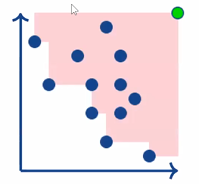
\includegraphics[width=0.3\linewidth]{images/hypervolume_2D.PNG}
    \caption{Пример:2D}
    \label{fig:mpr}
    
\end{center}
\end{figure}

\begin{figure}[!ht]
Однако для многомерной проблемы гипероъём справляется лучше, чем crowding distance.
Это связано с тем, что сложность вычисления crowding distance растет вместе с количеством измерений пространства. Гиперобъём в этом плане имеет константу.\\
Гиперобъём выделяет решения, которые доминируются на X. Благодаря этому мы уже получаем ранжированное множество точек, из которых можем выбрать оптимальное решение. 
\begin{center}
    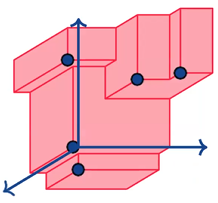
\includegraphics[width=0.3\linewidth]{images/hypervolume_3D.PNG}
    \caption{Пример:3D}
    \label{fig:mpr}
    
\end{center}
\end{figure}

Если существует некоторое решение, которое не доминирует $R$, тогда выделенный объём не будет работать, т.к. объём будет неоднозначным и будет некачественным.\\
\\
\\

Преимущества\\
- Полный порядок: любые два множества точек сравнимы\\
- Сильно коррелирует с отношением доминирования:
$A ≺ B → HV(A) > HV(B)$\\

Недостатки\\
- Вычисление гиперобъема NP-трудно\\
- $O N(logN)^_{max(1,\frac{(K −1)}{2})}$ для $N$ точек в $K$-мерном пространстве\\
- Весьма быстро для небольших размерностей\\
Может быть экспонентой от размера описания $NK$: все плохо, когда K большое\\
- $#P$-трудно для точного вычисления, NP-трудно для аппроксимации\\

Simple Indicator-Based Evolutionary Algorithm (SIBEA)\\
Поддерживаем популяцию недоминированных решений размера не более N\\
На каждой итерации:\\
- Генерируем одно новое решение (с использованием операторов
мутации, скрещивания и т.д.)\\
- Если оно не доминируется ни одним решением из популяции,\\
добавляем его в популяцию
- Если какие-то решения в популяции доминируются новым решением,
удаляем эти решения из популяции\\
- Если размер популяции равен N + 1, удаляем то из решений, без которого
гиперобъем популяции (или другой индикатор) максимален. Удаляем решение, без которого сохранится максимизация индикаторной функции (гиперобъём в данном случае).
